\documentclass[twocolumn]{extarticle}
\usepackage{fontspec}   %加這個就可以設定字體
\usepackage{xeCJK}       %讓中英文字體分開設置
%\usepackage{indentfirst}
\usepackage{listings}
\usepackage[newfloat]{minted}
\usepackage{float}
\usepackage{graphicx}
\usepackage{caption}
\usepackage{fancyhdr}
\usepackage{hyperref}
\usepackage{amsmath}
\usepackage{multirow}
\usepackage[dvipsnames]{xcolor}
\usepackage{graphicx}
\usepackage{tabularx}
\usepackage{booktabs}
\usepackage{caption}
\usepackage{subcaption}
\usepackage{pifont}
\usepackage{amssymb}
\usepackage{titling}

\usepackage{pdftexcmds}
\usepackage{catchfile}
\usepackage{ifluatex}
\usepackage{ifplatform}

\usepackage[breakable, listings, skins, minted]{tcolorbox}
\usepackage{etoolbox}
\setminted{fontsize=\footnotesize}
\renewtcblisting{minted}{%
    listing engine=minted,
    minted language=python,
    listing only,
    breakable,
    enhanced,
    minted options = {
        linenos, 
        breaklines=true, 
        breakbefore=., 
        % fontsize=\footnotesize, 
        numbersep=2mm
    },
    overlay={%
        \begin{tcbclipinterior}
            \fill[gray!25] (frame.south west) rectangle ([xshift=4mm]frame.north west);
        \end{tcbclipinterior}
    }   
}

\usepackage[
top=1.5cm,
bottom=1.5cm,
left=1.5cm,
right=1.5cm,
includehead,includefoot,
heightrounded, % to avoid spurious underfull messages
]{geometry} 

\usepackage[
    backend=biber,
    style=ieee,
    natbib=true,
    doi=true,
    eprint=false
]{biblatex}
\addbibresource{hw2.bib}

\newenvironment{code}{\captionsetup{type=listing}}{}
\SetupFloatingEnvironment{listing}{name=Code}
\usepackage[moderate]{savetrees}


\title{AI Capstone: Project 2 Report}
\author{110550088 李杰穎}
\date{\today}


\setCJKmainfont{Noto Serif TC}


\ifwindows
\setmonofont[Mapping=tex-text]{Consolas}
\fi

\XeTeXlinebreaklocale "zh"             %這兩行一定要加,中文才能自動換行
\XeTeXlinebreakskip = 0pt plus 1pt     %這兩行一定要加,中文才能自動換行

% \setlength{\parindent}{0em}
\setlength{\parskip}{0.75em}
\renewcommand{\baselinestretch}{1.25}
\setlength{\droptitle}{-10em}   % This is your set screw
\setlength{\columnsep}{2em}

\begin{document}

\maketitle

\section{Methods}

\subsection{Minimax and Expectimax}

Although Minimax and Expectimax algorithms are the classic algorithms that will be first considered when implementing a two-player gaming agent. However, when we try to apply the algorithms in the game of this project. One can observe that it may be really difficult for these algorithms to play some good moves. Because we only get the score (or reward) until the game is ended. Furthermore, this game didn't have the process of building up the advantage. The player can act like it might lose the game at first, but win the game eventually.

In conclusion, after my own analyzing, I think Minimax and Expectimax algorithms might not performing very well in this game. Therefore, I didn't implement these algorithms.

\subsection{MCTS}
Monte-Carlo Tree Search (MCTS) is a search algorithm that uses the UCT formula (\autoref{eq: uct}) for selection, followed by expansion and simulation from the selected node, and finally backpropagation of the simulation results to the nodes along the path. These steps constitute one iteration, and by adjusting the number of iterations, the execution time of MCTS algorithm can be controlled. This feature makes MCTS a suitable search algorithm for many games with limited total thinking time, such as Go, NoGo and the game in this project.

The four phases of MCTS are:

\begin{enumerate}
\item \textbf{Selection:} Starting from root \textbf{R} and select successive child nodes until a leaf node \textbf{L} is reached. The root is the current game state and a leaf is any node that has a potential child from which no simulation (playout) has yet been initiated. Selection is actually a process of \textbf{exploration} vs \textbf{exploitation}. Exploration is a long-term process, with a risky, uncertain outcome and exploitation is short-term, with immediate, relatively certain benefits. This process is being control by the UCT (Upper Confidence Bound 1 applied to trees) formula,

\begin{equation}
\frac{w_i}{n_i}+c\,\sqrt{\frac{\ln N_i}{n_i}}
\label{eq: uct}
\end{equation}

where $w_i$ is the total score (or reward or wins) for the node considered after the $i^{th}$ move, $n_i$ is the number of simulation for the node considered after the $i^{th}$ move, $N_i$ is the total number of simulations for the parent node of the one considered after the $i^{th}$ move and $c$ is the exploration parameter, theoretically equals to $\sqrt{2}$, but often chosen empirically. In the experiments, I will test different $c$ and compared the final win rate.

\item \textbf{Expansion:} Unless \textbf{L} ends the game decisively (e.g. win/loss/draw) for either player, create one (or more) child nodes and choose node \textbf{C} from one of them. Child nodes are any valid moves from the game position defined by \textbf{L}.
\item \textbf{Simulation (Rollout):} Complete one random playout from node \textbf{C}. A playout may be as simple as choosing uniform random moves until the game is decided.
\item \textbf{Backpropagation:} Use the result of the rollout to update information in the node on the path from \textbf{C} to \textbf{R}.
\end{enumerate}

Finally, it is worth noting that when selecting the best next move, MCTS chooses the node that has been visited the most times.

\begin{figure}[H]
\centering
\includegraphics[width=0.95\linewidth]{"img/mcts"}
\caption{Monte-Carlo Tree Search}
\label{fig:mcts}
\end{figure}

\subsection{Parallelization of MCTS}

MCTS is a powerful algorithm, it used a large number of simulations to estimate the best moves in the search tree. Therefore, if we can complete more simulations in a same time period, then the estimation will be more accurate, and consequently, the performance of the game agent will better.

Naturally, when it comes to complete more simulations, parallelization is the first method that will comes to our mind. 
In \cite{10.1007/978-3-540-87608-3_6}, the authors mentioned that there are four type of parallel MCTS, which are leaf parallelization, root parallelization, tree parallelization with global and local mutex, as shown in \autoref{fig:parallel-mcts}. 

Also, in \cite{5654650}, the authors test the above four methods, and found root parallelization is the best method among the four, and also, it is really easy to implement. Therefore, I will choose root-parallelization MCTS in this project to make the game agent better. Root parallelization is done by create multiple search tree, and let each thread do separate MCTS on the tree. When the searching is over, combined the searching results of all search tree and choose the node with highest visit count.

\begin{figure}[H]
\centering
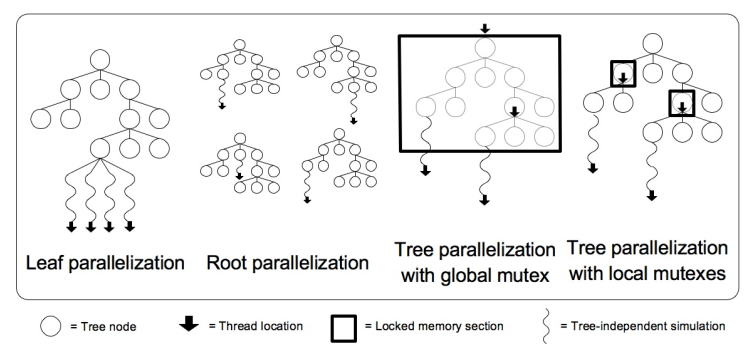
\includegraphics[width=0.95\linewidth]{img/parallel-mcts}
\caption{Four kinds of parallel MCTS, from \cite{10.1007/978-3-540-87608-3_6}.}
\label{fig:parallel-mcts}
\end{figure}


\section{Experiments \& Results}

In this section, I talk about the experiments I conduct, and the results will be shown in the next section.

Because I only implement MCTS algorithm, for algorithms comparison, I will compare parallel, non-parallel MCTS with same parameters. For parameters comparison, I will compare the exploration constant $c$, maximum search time $T$ and number of thread $m$.

Noted that all the experiments in this section has the configurations below:

\begin{enumerate}
\item Number of node: $12 \tilde 32$
\item Maximum thinking time: 0.5 second
\item Board Shape: randomly generate
\end{enumerate}

\subsection{Experiments against Random Player}

In this section, I use non-parallel MCTS with $c=\sqrt{2}$ to play against random player. In order to better estimate the real strength of MCTS and random player, I first conducted 50 games with MCTS agent as first player and later another 50 games with random agent as first player.

Noted that the thinking time for MCTS is 0.5 second, and the maximum number of iterations is 13500. As for the board configuration, the number of node is randomly between 12 and 32.

\begin{table}[H]
\centering
\caption{The number of winning games of MCTS and random agent. First 50 games are MCTS agent as first player and the last 50 games are random agent as first player.}
\label{tab:random}
\begin{tabular}{@{}cccc@{}}
\toprule
\textbf{Method}   & \textbf{First 50} & \textbf{Last 50} & \textbf{Win Rate} \\ \midrule
Non-parallel MCTS & 50                & 50               & 100 \%\\
Random            & 0                 & 0                & 0 \% \\ \bottomrule
\end{tabular}
\end{table}

As in \autoref{tab:random}, non-parallel MCTS beat random agent entirely, win all 100 games in my experiments. This results also shows that play this games randomly is a really bad strategy.

\subsection{Experiments about Parallelization}

Because a non-parallel MCTS can beat random agent easily, the only way to compare the strength of two agents is to let these two agents play against each other. \autoref{tab:para} shows the results of non-parallel MCTS and parallel MCTS with threads number equals to 3, the win rate of MCTS with $m=3$ is a little bit higher than MCTS with $m=1$, which is not surprising, because the total number of simulations of each moves is roughly 3 times higher. The fundamental of MCTS is by huge number of simulations to approach real results. Therefore, more simulations mean higher performance.

\begin{table}[H]
\centering
\caption{The number of winning games of different 1 and 3 threads. First 50 games are MCTS with 1 thread as first player and the last 50 games are MCTS with 3 threads as first player.}
\label{tab:para}
\begin{tabular}{@{}cccc@{}}
\toprule
\textbf{Method}   & \textbf{First 50} & \textbf{Last 50} & \textbf{Win Rate} \\ \midrule
MCTS w/ $m=1$ & 21                & 23               & 44 \%\\
MCTS w/ $m-3$            & 29                 & 27                & 56 \% \\ \bottomrule
\end{tabular}
\end{table}



\subsection{Experiments about Exploration Parameter $c$}

In many paper, including \cite{10.1007/978-3-540-87608-3_6}, use different $c$ other than $\sqrt{2}$, for example, 0.35. Therefore, I compare the MCTS with different $c$. Noted that these two agents both have $m=3$. 

In \autoref{tab:c}, we can observe that the win rate of MCTS with $c=0.35$ is actually much higher than the one with $c=\sqrt{2}$. This results is really surprised me, before conducting the experiments, I thought the win rate between the two won't have huge difference. But in fact, $c$ can effect the strength of MCTS very much. I think the reason why smaller $c$ has better strength is in this game, drawing lines in different location doesn't effect the final results very much, therefore focused on the node with higher win rate is better for the final results.

\begin{table}[H]
\centering
\caption{The number of winning games of different $c$. First 50 games are MCTS with $c=\sqrt{2}$ as first player and the last 50 games are MCTS with $c=0.35$ as first player.}
\label{tab:c}
\begin{tabular}{@{}cccc@{}}
\toprule
\textbf{Method}   & \textbf{First 50} & \textbf{Last 50} & \textbf{Win Rate} \\ \midrule
MCTS w/ $c=\sqrt{2}$ & 12                & 17               & 29 \%\\
MCTS w/ $c=0.35$            & 38                 & 33                & 71 \% \\ \bottomrule
\end{tabular}
\end{table}

\section{Future Works}

When researching on the internet, I found that there has a framework called \textit{alpha-zero-general}, which is a Python library that provides the architectures of alpha-zero and various game. This framework can be easily adapted to the game in the project. Maybe this method can achieve better strength.


\printbibliography

\end{document}
